\section{Sonstiges}
\label{sec:Sonstiges}

\subsection{Umrechung von Datengrößen}
\label{sec:Datengroessen}

\begin{center}
	\begin{tikzpicture}[align=center, 
		node distance= 1cm,
		node/.style={rectangle, inner sep=10, draw}]
		
		\node (B) [node] {B};
	
		\node (kB10) [node, above right=of B]{kB\\$10^{3}$};
		\node (MB10) [node, right=of kB10] {MB\\$10^{6}$};
		\draw[->] (kB10) to [out=80, in=100] node[above] {$:10^{3}$} (MB10);
		\draw[->] (MB10) to [out=250, in=290] node[below] {$*10^{3}$} (kB10);
		\node (GB10) [node, right=of MB10] {GB\\$10^{9}$};
		\draw[->] (MB10) to [out=80, in=100] node[above] {$:10^{3}$} (GB10);
		\draw[->] (GB10) to [out=250, in=290] node[below] {$*10^{3}$} (MB10);
		\node (TB10) [node, right=of GB10] {TB\\$10^{12}$};
		\draw[->] (GB10) to [out=80, in=100] node[above] {$:10^{3}$} (TB10);
		\draw[->] (TB10) to [out=250, in=290] node[below] {$*10^{3}$} (GB10);
		\node (PB10) [node, right=of TB10] {PB\\$10^{15}$};
		\draw[->] (TB10) to [out=80, in=100] node[above] {$:10^{3}$} (PB10);
		\draw[->] (PB10) to [out=250, in=290] node[below] {$*10^{3}$} (TB10);
		
		\node (KiB2) [node, below right=of B]{KiB\\$2^{10}$};
		\node (MiB2) [node, right=of KiB2] {MiB\\$2^{20}$};
		\draw[->] (KiB2) to [out=80, in=100] node[above] {$:2^{10}$} (MiB2);
		\draw[->] (MiB2) to [out=250, in=290] node[below] {$*2^{10}$} (KiB2);
		\node (GiB2) [node, right=of MiB2] {GiB\\$2^{30}$};
		\draw[->] (MiB2) to [out=80, in=100] node[above] {$:2^{10}$} (GiB2);
		\draw[->] (GiB2) to [out=250, in=290] node[below] {$*2^{10}$} (MiB2);
		\node (TiB2) [node, right=of GiB2] {TiB\\$2^{40}$};
		\draw[->] (GiB2) to [out=80, in=100] node[above] {$:2^{10}$} (TiB2);
		\draw[->] (TiB2) to [out=250, in=290] node[below] {$*2^{10}$} (GiB2);
		\node (PiB2) [node, right=of TiB2] {PiB\\$2^{50}$};
		\draw[->] (TiB2) to [out=80, in=100] node[above] {$:2^{10}$} (PiB2);
		\draw[->] (PiB2) to [out=250, in=290] node[below] {$*2^{10}$} (TiB2);
		
		\draw[->] (B) to [out=120, in=150] node[above left] {$:10^{3}$} (kB10);
		\draw[->] (kB10) to [out=250, in=10] node[above left] {$*10^{3}$} (B);
		
		\draw[->] (B) to [out=340, in=100] node[below left]{$:2^{10}$} (KiB2);
		\draw[->] (KiB2) to [out=200, in=250] node[below left] {$*2^{10}$} (B);
	\end{tikzpicture}
\end{center}

\begin{center}
	\begin{tikzpicture}[align=center, 
		node distance= 2cm,
		node/.style={rectangle, inner sep=10, draw}]
		
		\node (Byte)[node] {Byte};
		\node (Bit) [node, right=of Byte]{Bit};
		
		\draw[->] (Byte) to [out=80, in=100] node[above] {$*8$} (Bit);
		\draw[->] (Bit) to [out=250, in=290] node[below] {$:8$} (Byte);
		
	\end{tikzpicture}
\end{center}


\subsection{Berechnung von Bildgrößen}
\label{sec:Bildgroesse}

Farbtiefe, RGB, Pixel, DPI, etc.

\paragraph{DPI} Dots per Inch (Pixel pro Inch)


\subsection{Netzplan}
\label{sec:Netzplan}

\quelle{MODU learn}{Netzplan}

Die Basis für den Netzplan ist ein Prozess, der aus insgesamt sieben Teilschritten besteht. Zu jedem Schritt sind sowohl die Dauer als auch die vorher abzuschließenden Aufgaben bekannt:

\begin{center}
	\bgroup
	\setlength{\tabcolsep}{1em}
	\def\arraystretch{1.5}
	\begin{tabular}{|l|l|l|}
		\hline
		\rowcolor{tableLightGray}Prozessschritt & Dauer in Stunden & Vorher zu beenden \\
		\hline
		A & 2 & - \\
		\hline
		B & 4 & A \\
		\hline
		C & 3 & B \\
		\hline
		D & 2 & B \\
		\hline
		E & 1 & C,D \\
		\hline
		F & 4 & C \\
		\hline
		G & 5 & E,F \\
		\hline
	\end{tabular}
	\egroup
\end{center}

Diese Schritte müssen gleich in Form von sogenannten Knoten dargestellt und miteinander verbunden werden. Daher sollten wir uns als zusätzliche Vorbereitung den grundlegenden Aufbau eines Knotens anschauen. Er weist die folgende Struktur auf:

\begin{center}
	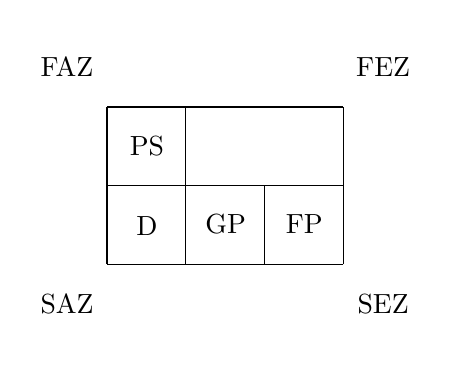
\begin{tikzpicture}[
		align=center,
		every node/.style={minimum height = 1cm, minimum width = 1cm}]
		
		\draw (0,0) node[anchor=north east]{SAZ} -- (3,0);
		\draw (3,0) node[anchor=north west]{SEZ} -- (3,2);
		\draw (3,2) node[anchor=south west]{FEZ} -- (0,2);
		\draw (0,2) node[anchor=south east]{FAZ} -- (0,0);
		
		\draw (1,0) node[anchor=south west]{GP} -- (1,2);
		\draw (2,0) node[anchor=south west]{FP} -- (2,1);
		\draw (0,1) node[anchor=south west]{PS} node[anchor=north west]{D} -- (3,1);
		
	\end{tikzpicture}
\end{center}

\textbf{PS} = Prozessschritt (in unserem Fall A bis F)\\
\textbf{D} = Dauer des jeweiligen Vorgangs\\
\textbf{FAZ} = Frühester Anfangszeitpunkt, zu dem der Prozessschritt begonnen werden kann\\
\textbf{FEZ} = Frühester Endzeitpunkt, zu dem der Prozessschritt abgeschlossen werden kann\\
\textbf{SAZ} = Spätester Anfangszeitpunkt, um den Gesamtprozess planmäßig beenden zu können\\
\textbf{SEZ} = Spätester Endzeitpunkt, zu dem ein Schritt abgeschlossen sein muss, um den geplanten Abschlusstermin nicht zu gefährden\\
\textbf{GP} = Gesamtpuffer, der genutzt werden kann, bevor der pünktliche Abschluss des Gesamtprozesses gefährdet wird\\
\textbf{FP} = Freier Puffer, der zur Verfügung steht, bevor der unmittelbar folgende Prozessschritt beeinflusst wird\\

\subsubsection{Schritt 1: Knoten verknüpfen}

Zuerst erstellst Du einen vorläufigen Netzplan, in dem einerseits die Prozessschritte und ihre Abhängigkeiten abgebildet sind und andererseits die jeweilige Dauer der Knoten. Das sieht für unseren konkreten Fall dann so aus:


